The functionality of the FPGA timetagger is primarily accessed through
two graphical interfaces provided by {\tt timetag\_tools}: {\tt
 timetag\_ui} and {\tt timetag\_seq\_ui}. These are both installed in
the system application list as shown in \ref{Fig:Dash}.

\section{Timetagger UI}

The timetagger interface, {\tt timetag\_ui}, is a graphical frontend to
the device's timetagging functionality.

\begin{figure}
  \center
  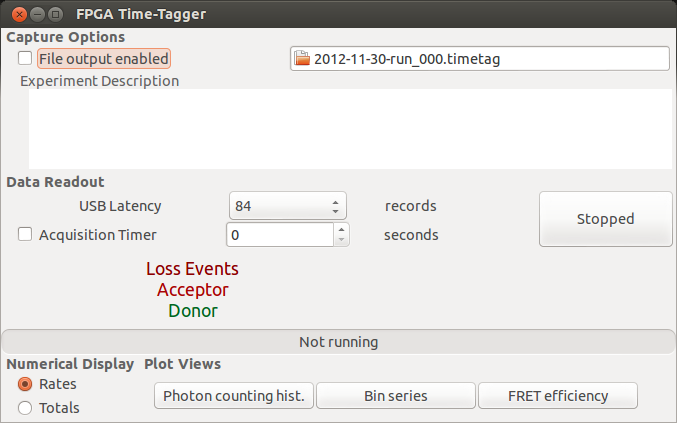
\includegraphics[scale=0.5]{timetag-window.png}
  \caption{The main window of {\tt timetag\_ui}.}
  \label{Fig:MainWindow}
\end{figure}

The main window the timetagger interface display 

